% This section contains notes on "Configure Microsoft Azure AD Privileged Identity Management" relevant subjects %
\subsubsection{Privileged identity management}
Privileged identity management seeks to accomplish:
\begin{itemize}
\item Integrated access reviews 
\item Manage risk : least privilege access
	\begin{itemize}	
	\item Just-in-time access
	\item Request approval workflows
	\end{itemize}
\item Address compliance and governance
\item Prevention of malicious activities in real time
\end{itemize}

\textbf{Setup}
\begin{enumerate}
\item Sign in. \textit{As global administrator.}
\item Navigate to PIM service. \textit{Click All services and find the Azure AD Privileged Identity Management service.}
\item Setup MFA for account. \textit{If not already done.}
\item Consent to PIM. \textit{Automatically assigned the Security Administrator and Privileged Role Administrator roles.}
\item Verify identify. \textit{With MFA.}
\end{enumerate}

\textbf{Deployment} 
\begin{enumerate}
\item Identify stakeholders
\item Enable Privileged Identity Management
\item Enforce principle of least privilege
	\begin{enumerate}
	\item Understand the granularity of the roles
	\item List who has privileged roles in your organization
	\item Reduce the amount of Global Administrators. \textit{Consider automating with acess review}.
	\item Reduce other administrators. \textit{Consider automating with acess review}.
	\end{enumerate}
\item Decide which role assignments should be protected by Privileged Identity Management
	\begin{enumerate}
	\item Should be atleast Global Administrators and Security Administrators
	\item All guest users
	\item Owner roles and User Access Administrator roles of all subscriptions/resources
	\end{enumerate}
\item Decide which role assignments should be permanent or eligible
	\begin{enumerate}
	\item Two break-glass emergency access accounts
	\end{enumerate}
\item Draft your Privileged Identity Management settings
\end{enumerate}
\begin{enumerate}
\item Use Privileged Identity Management alerts to safeguard your privileged access
\item Set up recurring access reviews to regularly audit your organization’s privileged identities
	\begin{enumerate}
	\item Quarterly access reviews for all your Azure AD and Azure resource roles
	\item Secondary email address for all accounts with privileged role assignments that are not linked to a regularly checked email address
	\end{enumerate}
\item Get the most out of your audit log to improve security and compliance
	\begin{enumerate}
	\item Read all audit events on a weekly basis and export your audit events on a monthly basis
	\item Use Azure log monitoring to archive audit events in an Azure storage account for the need of security and compliance
	\end{enumerate}
\end{enumerate}

\textbf{Features} \\
\begin{tabular}{p{3cm} p{12cm}}
\textbf{Tasks} \\
My roles & List of eligible\footnote{A role assignment that requires a user to perform one or more actions to use the role. If a user has been made eligible for a role, that means they can activate the role when they need to perform privileged tasks. These can be viewed and activated here.} and active roles assigned to you. \\
My requests & Pending requests to activate eligible role assignments. \\
Approve requests & Requests to activate eligible roles, that you are designated to approve. \\
Review access & Active access reviews you are assigned to complete, whether you're reviewing access for yourself or someone else. \\
\textbf{Manage} \\
Azure AD roles & Dashboard and settings to manage Azure AD role assignments. \newline \textit{Only for privileged role administrators.} \\
Azure resources & Dashboard and settings to manage Azure resource role assignments. \newline \textit{Only for privileged role administrators.} \\
\end{tabular}

\textbf{Restrictions} \\
Privileged Identity Management does not allow the management for all roles. Specifically some classic subscription administrator roles and some Exchange and Sharepoint roles.
\begin{itemize}
\item Account Administrator
\item Service Administrator
\item Co-Administrator
\item Exchange Online roles 
\item SharePoint Online roles
\end{itemize}
Exchange Administrator and SharePoint Administrator are available, but can experience delays. 

\begin{figure}[!h]
\centering
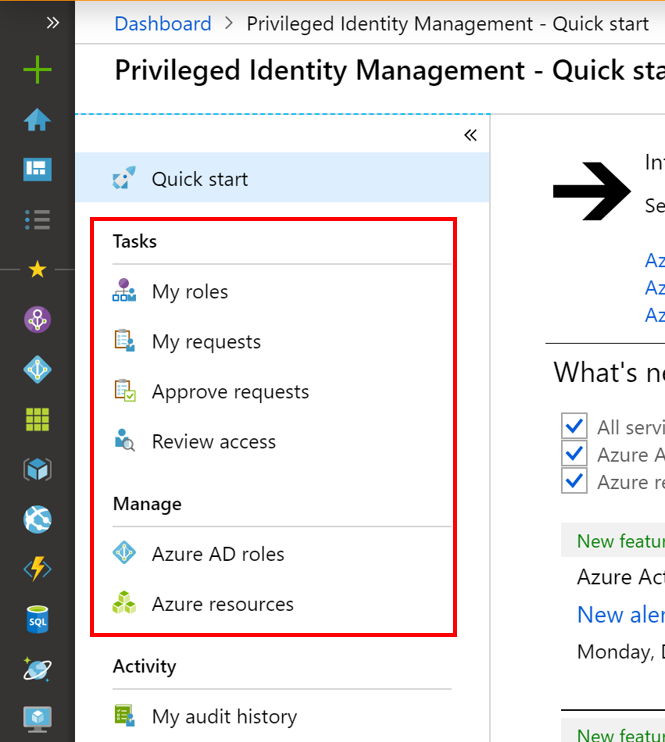
\includegraphics[width=0.5\textwidth]{pim-quickstart-tasks.png}
\caption{Privileged Identity Management - Quick start}
\label{fig:azure-connect-accounts}
\end{figure}

Depending on the Privileged Identity Management settings configured for the role, the user must complete certain steps (such as performing multi-factor authentication, getting approval, or specifying a reason.)

\textbf{License requirements}
\begin{itemize}
\item Azure AD Premium P2
\item Enterprise Mobility + Security (EMS) E5
\item Microsoft 365 M5
\end{itemize}

\textbf{User roles with Privileged Identity Management access}
Each administrator or user who interacts with or receives a benefit from Privileged Identity Management must have a license. Examples include:
\begin{itemize}
\item Administrators
	\begin{itemize}
	\item with Azure AD roles managed using PIM
	\item Azure resource roles managed using PIM
	\item assigned to the Privileged Role Administrator role
	\end{itemize}
\item Users
	\begin{itemize}
	\item assigned as eligible to Azure AD roles managed using PIM
	\item able to approve/reject requests in PIM
	\item assigned to an Azure resource role with just-in-time or direct (time-based) assignments
	\item assigned to an access review
	\item who perform access reviews
	\end{itemize}
\end{itemize}

\textbf{Trivia and quirks} 
\begin{enumerate}
\item First person to use Privileged Identity Management in your directory, is automatically assigned the Security Administrator and Privileged Role Administrator roles
\item Only \textit{organizational} accounts, with Global Administrator role, can enable Privileged Identity Management for a directory
\end{enumerate}

\subsubsection{Access review}
